\section{Introduction}

Predictive modeling is a well researched method for building optimization heuristics that often exceed human experts and reduces development time~\cite{Micolet2016,Wang2014c,Magni2014,Cummins2016,Wang2009,Wen2015,Wang2010,Falch2015,Collins2012,Leather2014,Ogilvie2014a}. Figure~\ref{fig:training-a-predictive-model} shows the process by which these models are trained. A set of training programs are identified that are expected to be representative of the application domain. The programs are compiled and executed with different parameter values for the target heuristic, to determine which are the best values for each training program. Each program is also summarized by a vector of features which describe the information that is expected to be important in predicting the best heuristic parameter values. These training examples of program features and desired heuristic values are used to create a machine learning model which, when given the features from a new, unseen program, can predict good heuristic values for it.

\begin{figure}
  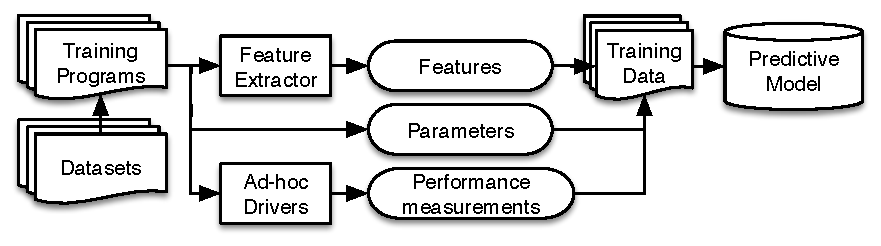
\includegraphics[width=\columnwidth]{img/overview-a}%
  \caption{Training a predictive model.}%
  \label{fig:training-a-predictive-model}
\end{figure}

It is common for feature vectors to contain dozens of elements. This means that a large volume of training data is needed to have an adequate sampling over the feature space. Without it, the machine learned models can only capture the coarse characteristics of the heuristic, and new programs which do not lie near to training points may be wrongly predicted. The accuracy of the machine learned heuristic is thus limited by the sparsity of the training points.

There have been efforts to solve this problem using templates. The essence of the approach is to construct a probabilistic grammar with embedded semantic actions that defines a language of possible programs. New programs may be created by sampling the grammar and, through setting probabilities on the grammar productions, the sampling is biased towards producing programs from one part of the space or another. This technique is potentially completely general, since a grammar can theoretically be constructed to match any desired program domain. However, despite being theoretically possible, it is not easy to construct grammars which are both suitably general and also produce programs that are in any way similar to human written programs. It has been shown to be successful over a highly restricted space of stencil benchmarks with little control flow or program variability~\cite{Falch2015,Cummins2016}. But, it is not clear how much effort it will take, or even if it is possible for human experts to define grammars capable of producing human like programs in more complex domains.

By contrast, our approach does not require an expert to define what human programs look like. Instead, we automatically infer the structure and likelihood of programs over a huge corpus of open source projects. From this corpus, we learn a probability distribution over sets of characters seen in human written code. Later, we sample from this distribution to generate new random programs which, because the distribution models human written code, are indistinguishable from human code. We can then populate our training data with an unbounded number of human like programs, covering the space far more finely than either existing benchmark suites or even the corpus of open source projects. Our approach is enabled by two recent developments:

The first is the breakthrough effectiveness of deep learning for modeling complex structure in natural languages~\cite{Graves2013,Sutskever2014}. As we show, deep learning is capable not just of learning the macro syntactical and semantic structure of programs, but also the nuances of how humans typically write code. It is truly remarkable when one considers that it is given no prior knowledge of the syntax or semantics of the language.

The second is the increasing popularity of public and open platforms for hosting software projects and source code. This popularity furnishes us with the thousands of programming examples that are necessary to feed into the deep learning. These open source examples are not, sadly, as useful for directly learning the compiler heuristics since they are not presented in a uniform, runnable manner, nor do they typically have extractable test data. Preparing each of the thousands of open source projects to be directly applicable for learning compiler heuristics would be an insurmountable task. In addition to our program generator, CLgen, we also provide an accompanying host driver which generates datasets for, then executes and profiles synthesized programs.

We make the following contributions:%
\begin{itemize}
  \item We are the first to apply deep learning over source codes to synthesize compilable, executable benchmarks.%
  \item A novel tool CLgen\footnote{\url{https://github.com/ChrisCummins/clgen}} for general-purpose benchmark synthesis using deep learning. CLgen automatically and rapidly generates thousands of human like programs for use in predictive modeling.%
  \item We use CLgen to automatically improve the performance of a state of the art predictive model by $1.27\times$, and expose limitations in the feature design of the model which, after correcting, further increases performance by $4.30\times$.%
\end{itemize}
